\chapter{Manual de Funcionamento do Palabos Acoustic}

Para executar o \citeonline{palabos_acoustic} é preciso dos seguintes \textit{softwares} básicos instalados como pré-requisitos:

\begin{itemize}
  \item sistema operacional linux Ubuntu 16.04 ou CentOS 7.2;
  \item compilador de C++ do tipo g++ 4.8;
  \item biblioteca de processamento paralelo Open MPI 1.10. 
\end{itemize}

Para cada novo modelo é preciso criar uma pasta com o nome do modelo contendo o arquivo de compilação \textbf{Makefile} e o código fonte do modelo numérico escrito em C++ com extenção \textbf{.cpp}. No arquivo \textbf{Makefile} é possível configurar aonde se encontra a instalação do Palabos, arquivo do modelo numérico com extenção \textbf{.cpp}, opções de depuração e opções de paralelização. No arquivo de extenção \textbf{.cpp} se encontra o código fonte do modelo numérico a ser simulado e o mesmo é composto de acordo com os procedimentos do fluxograma da Figura \ref{fig:palabos_fluxo}.


\begin{figure}[ht!]
\centering
  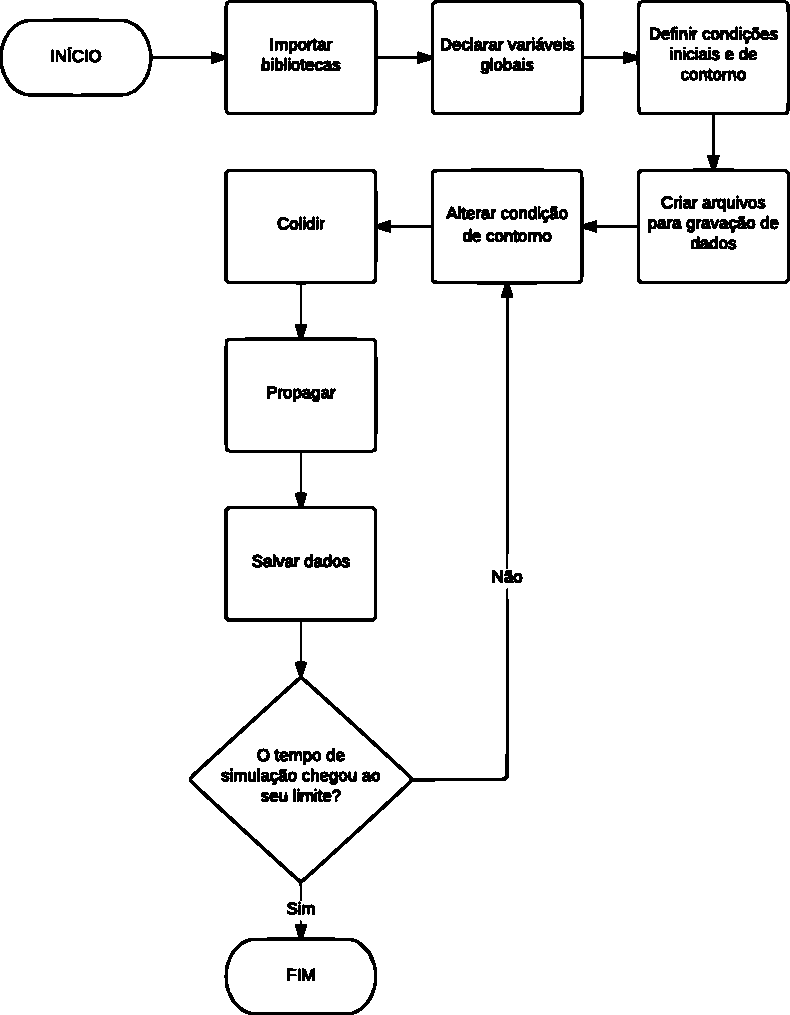
\includegraphics[width=.8\linewidth]{figuras/palabos_modelo_fluxo.pdf}
  \caption[Fluxograma de um modelo numérico no Palabos]{Fluxograma geral de um código fonte de um modelo numérico no Palabos.}
  \label{fig:palabos_fluxo}
\end{figure}

Como é mostrado na Figura \ref{fig:palabos_fluxo}, todo código de modelo numérico no Palabos possui os seguintes procedimentos:

\begin{itemize}
  \item importar bibliotecas: nesse procedimento são importadas as bibliotecas que contêm as funções e classes que serão usadas ao longo do processamento do modelo. Normalmente são bibliotecas do próprio Palabos ou bibliotecas com funções matemáticas;
  \item definir variáveis globais: normalmente nessa etapa são definidas valores de pré-processamento como o tamanho do domínio, valores macroscópicos do fluido como número de Reynolds, tempo total de simulação, viscosidade cinemática e o tipo de modelo LBM;
  \item definir condições iniciais e de contorno: nessa etapa a malha do domínio é consolidada, valores de densidade e velocidade são atribuídas para cada célula do domínio e condições de contorno são impostas;
  \item criar arquivos para gravação de dados: são criados ponteiros e arquivos de diversas extensões para que os dados sejam gravados;
  \item alterar condição de contorno: nessa etapa o modelo numérico entra no \textit{loop} de iterações e se necessário as condições de contorno são alteradas para, por exemplo, que um \textit{sweep} possa ser imposto;
  \item colidir: nessa etapa o operador de colisão é calculado e somado com as funções de distribuição de cada célula;
  \item propagar: os valores das funções de distribuição são propagados para células vizinhas;
  \item salvar dados: os dados normalmente de pressão e velocidades são salvos para pós-processamento. 
\end{itemize}
E assim o ciclo de procedimentos dentro do \textit{loop} é executado até que o número de iterações alcance o número máximo de tempo definido no início do programa.

Para execução é preciso efetuar os seguintes comandos no terminal linux dentro da pasta do modelo numérico:
\begin{itemize}
  \item compilação do código de extenção \textbf{.cpp} para formato binário em linguagem de máquina:
  \begin{lstlisting}[language=make, frame = single]
    $ make
  \end{lstlisting}
  \item execução do arquivo binário compilado:
  \begin{lstlisting}[language=make, frame = single]
    $ mpirun -np 
    <numero_de_processadores> 
    <nome_do_arquivo_compilado> 
    <parametros_de_entrada>
  \end{lstlisting}
  aplicando para o modelo numérico desse trabalho:
  \begin{lstlisting}[language=make, frame = single]
    $ mpirun -np 
    8
    duct_radiation_optimization
    20 0.15 1.99
  \end{lstlisting}
  tal que o raio do duto é 20 células, o mach do escoamento é 0.15 e 1.99 é a frequência de relaxação $1/\tau$. É possível também executar o Palabos com o \textit{script} \textbf{duct\_radiation\_init.m} na plataforma \citeonline{matlab} ou \citeonline{octave}. Para executar basta colocar esse \textit{script} dentro da pasta do modelo numérico e executar o seguinte comando no terminal do \citeonline{matlab} ou \citeonline{octave} dentro dessa pasta:
  \begin{lstlisting}[language=matlab, frame = single]
    >> duct_radiation_init 20 0.15 5042 8
  \end{lstlisting}
  tal que o raio do duto é 20 células, o mach do escoamento é 0.15, o número de Reynolds é 5042 e o 8 é a quantidade de processadores.
\end{itemize}
